\documentclass[tikz,border=2pt]{standalone}
\usepackage[tt=false,type1=true]{libertine}
\usetikzlibrary{arrows.meta,positioning}
\definecolor{accent}{HTML}{B03A2E}
\begin{document}
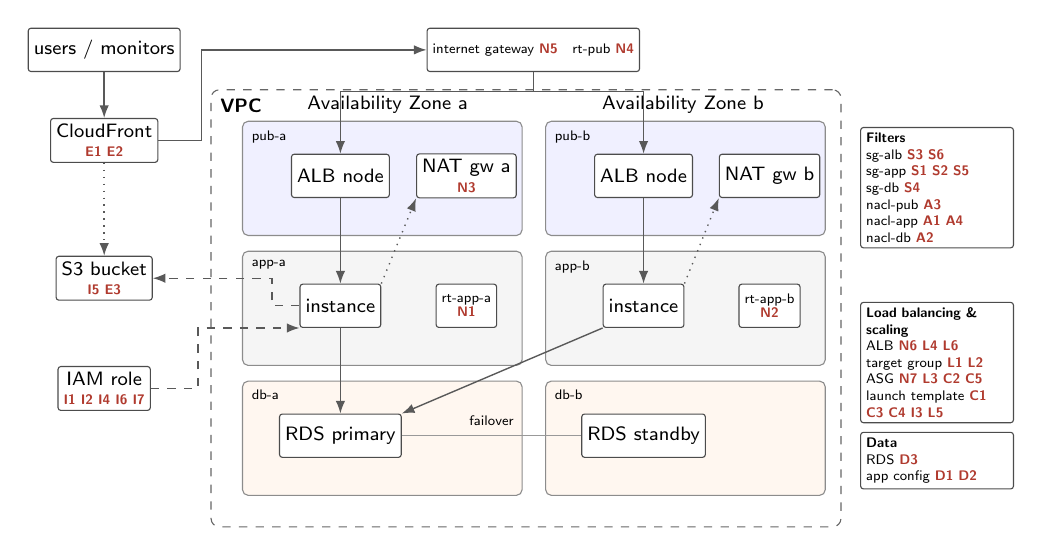
\begin{tikzpicture}[
  font=\sffamily\scriptsize,
  res/.style={draw=black!70, rounded corners=1pt, fill=white, align=center, inner sep=2pt, minimum height=0.55cm},
  sub/.style={draw=black!45, fill=#1, rounded corners=2pt, minimum width=3.55cm, minimum height=1.45cm},
  sub/.default={black!4},
  flt/.style={text=accent, font=\sffamily\tiny\bfseries},
  arr/.style={-{Latex[length=1.6mm]}, draw=black!65, line width=0.5pt},
  mon/.style={align=left, font=\sffamily\tiny}
]
% VPC frame
\node[draw=black!60, dashed, rounded corners=3pt, minimum width=8.0cm, minimum height=5.55cm, anchor=north west] (vpc) at (2.6,0.05) {};
\node[anchor=north west, font=\sffamily\scriptsize\bfseries] at (vpc.north west) {VPC};
\node[font=\sffamily\scriptsize] at (4.85,-0.15) {Availability Zone a};
\node[font=\sffamily\scriptsize] at (8.6,-0.15) {Availability Zone b};
% subnets
\node[sub=blue!6, anchor=north west] (puba) at (3.0,-0.35) {};
\node[sub=blue!6, anchor=north west] (pubb) at (6.85,-0.35) {};
\node[sub=black!4, anchor=north west] (appa) at (3.0,-2.0) {};
\node[sub=black!4, anchor=north west] (appb) at (6.85,-2.0) {};
\node[sub=orange!6, anchor=north west] (dba) at (3.0,-3.65) {};
\node[sub=orange!6, anchor=north west] (dbb) at (6.85,-3.65) {};
\node[anchor=north west, font=\sffamily\tiny] at (puba.north west) {pub-a};
\node[anchor=north west, font=\sffamily\tiny] at (pubb.north west) {pub-b};
\node[anchor=north west, font=\sffamily\tiny] at (appa.north west) {app-a};
\node[anchor=north west, font=\sffamily\tiny] at (appb.north west) {app-b};
\node[anchor=north west, font=\sffamily\tiny] at (dba.north west) {db-a};
\node[anchor=north west, font=\sffamily\tiny] at (dbb.north west) {db-b};
% public tier
\node[res] (albA) at (4.25,-1.05) {ALB node};
\node[res] (natA) at (5.85,-1.05) {NAT gw a\\[-1pt]\textcolor{accent}{\tiny\bfseries N3}};
\node[res] (albB) at (8.1,-1.05) {ALB node};
\node[res] (natB) at (9.7,-1.05) {NAT gw b};
% app tier
\node[res] (iA) at (4.25,-2.7) {instance};
\node[res] (iB) at (8.1,-2.7) {instance};
\node[res, font=\sffamily\tiny] (rta) at (5.85,-2.7) {rt-app-a\\[-1pt]\textcolor{accent}{\bfseries N1}};
\node[res, font=\sffamily\tiny] (rtb) at (9.7,-2.7) {rt-app-b\\[-1pt]\textcolor{accent}{\bfseries N2}};
% data tier
\node[res] (rdsA) at (4.25,-4.35) {RDS primary};
\node[res] (rdsB) at (8.1,-4.35) {RDS standby};
% cross-cutting labels inside VPC (right side panel)
\node[res, anchor=west, font=\sffamily\tiny, text width=1.8cm, align=left] (filters) at (10.85,-1.2) {%
  \textbf{Filters}\\
  sg-alb \textcolor{accent}{\bfseries S3 S6}\\
  sg-app \textcolor{accent}{\bfseries S1 S2 S5}\\
  sg-db \textcolor{accent}{\bfseries S4}\\
  nacl-pub \textcolor{accent}{\bfseries A3}\\
  nacl-app \textcolor{accent}{\bfseries A1 A4}\\
  nacl-db \textcolor{accent}{\bfseries A2}};
\node[res, anchor=north west, font=\sffamily\tiny, text width=1.8cm, align=left] (lb) at (10.85,-2.65) {%
  \textbf{Load balancing \& scaling}\\
  ALB \textcolor{accent}{\bfseries N6 L4 L6}\\
  target group \textcolor{accent}{\bfseries L1 L2}\\
  ASG \textcolor{accent}{\bfseries N7 L3 C2 C5}\\
  launch template \textcolor{accent}{\bfseries C1 C3 C4 I3 L5}};
\node[res, anchor=north west, font=\sffamily\tiny, text width=1.8cm, align=left] (data) at (10.85,-4.3) {%
  \textbf{Data}\\
  RDS \textcolor{accent}{\bfseries D3}\\
  app config \textcolor{accent}{\bfseries D1 D2}};
% gateway and route on the top edge
\node[res, font=\sffamily\tiny] (igw) at (6.7,0.55) {internet gateway \textcolor{accent}{\bfseries N5}\quad rt-pub \textcolor{accent}{\bfseries N4}};
% outside the VPC
\node[res] (cf) at (1.25,-0.6) {CloudFront\\[-1pt]\textcolor{accent}{\tiny\bfseries E1 E2}};
\node[res] (s3) at (1.25,-2.35) {S3 bucket\\[-1pt]\textcolor{accent}{\tiny\bfseries I5 E3}};
\node[res] (iam) at (1.25,-3.75) {IAM role\\[-1pt]\textcolor{accent}{\tiny\bfseries I1 I2 I4 I6 I7}};
\node[res] (users) at (1.25,0.55) {users / monitors};
% arrows (request path)
\draw[arr] (users) -- (cf);
\draw[arr] (cf.east) -- ++(0.55,0) |- (igw.west);
\draw[arr] (igw.south) -- ++(0,-0.25) -| (albA.north);
\draw[arr] (igw.south) -- ++(0,-0.25) -| (albB.north);
\draw[arr] (albA) -- (iA);
\draw[arr] (albB) -- (iB);
\draw[arr] (iA) -- (rdsA);
\draw[arr] (iB.south west) -- (rdsA.north east);
\draw[arr, dashed] (iA.west) -- ++(-0.35,0) |- (s3.east);
\draw[arr, dashed] (iam.east) -- ++(0.6,0) |- (iA.south west);
\draw[arr, dotted] (cf.south) -- (s3.north);
\draw[arr, dotted] (iA.north east) -- (natA.south west);
\draw[arr, dotted] (iB.north east) -- (natB.south west);
\draw[-, draw=black!40] (rdsA) -- node[above, font=\sffamily\tiny]{failover} (rdsB);
\end{tikzpicture}
\end{document}
